\documentclass[10pt]{beamer}\usepackage[]{graphicx}\usepackage{xcolor}
%% maxwidth is the original width if it is less than linewidth
%% otherwise use linewidth (to make sure the graphics do not exceed the margin)
\makeatletter
\def\maxwidth{ %
  \ifdim\Gin@nat@width>\linewidth
    \linewidth
  \else
    \Gin@nat@width
  \fi
}
\makeatother

\definecolor{fgcolor}{rgb}{0.345, 0.345, 0.345}
\newcommand{\hlnum}[1]{\textcolor[rgb]{0.686,0.059,0.569}{#1}}%
\newcommand{\hlstr}[1]{\textcolor[rgb]{0.192,0.494,0.8}{#1}}%
\newcommand{\hlcom}[1]{\textcolor[rgb]{0.678,0.584,0.686}{\textit{#1}}}%
\newcommand{\hlopt}[1]{\textcolor[rgb]{0,0,0}{#1}}%
\newcommand{\hlstd}[1]{\textcolor[rgb]{0.345,0.345,0.345}{#1}}%
\newcommand{\hlkwa}[1]{\textcolor[rgb]{0.161,0.373,0.58}{\textbf{#1}}}%
\newcommand{\hlkwb}[1]{\textcolor[rgb]{0.69,0.353,0.396}{#1}}%
\newcommand{\hlkwc}[1]{\textcolor[rgb]{0.333,0.667,0.333}{#1}}%
\newcommand{\hlkwd}[1]{\textcolor[rgb]{0.737,0.353,0.396}{\textbf{#1}}}%
\let\hlipl\hlkwb

\usepackage{framed}
\makeatletter
\newenvironment{kframe}{%
 \def\at@end@of@kframe{}%
 \ifinner\ifhmode%
  \def\at@end@of@kframe{\end{minipage}}%
  \begin{minipage}{\columnwidth}%
 \fi\fi%
 \def\FrameCommand##1{\hskip\@totalleftmargin \hskip-\fboxsep
 \colorbox{shadecolor}{##1}\hskip-\fboxsep
     % There is no \\@totalrightmargin, so:
     \hskip-\linewidth \hskip-\@totalleftmargin \hskip\columnwidth}%
 \MakeFramed {\advance\hsize-\width
   \@totalleftmargin\z@ \linewidth\hsize
   \@setminipage}}%
 {\par\unskip\endMakeFramed%
 \at@end@of@kframe}
\makeatother

\definecolor{shadecolor}{rgb}{.97, .97, .97}
\definecolor{messagecolor}{rgb}{0, 0, 0}
\definecolor{warningcolor}{rgb}{1, 0, 1}
\definecolor{errorcolor}{rgb}{1, 0, 0}
\newenvironment{knitrout}{}{} % an empty environment to be redefined in TeX

\usepackage{alltt}

\usepackage[english]{babel}
\usepackage[T1]{fontenc}
\usepackage[utf8]{inputenc}
\usepackage{amsmath}
\usepackage{array}
\usepackage{adjustbox}
\usepackage{xspace}
\usepackage{tikz}
\usetikzlibrary{shapes,arrows,backgrounds,fit,positioning,chains,shadows,decorations.pathmorphing,decorations.pathreplacing,matrix}
\usepackage{csquotes}
\usepackage{booktabs}
\usepackage{wasysym}
\usepackage[binary-units=true]{siunitx}
\usepackage{xcolor}
\usepackage{pifont}
\usepackage{dsfont}

\definecolor{tugreen}{cmyk}{0.57, 0, 1.00, 0}
\definecolor{tugreen1}{cmyk}{0.57, 0, 1.00, 0}
\definecolor{tugreen2}{HTML}{667E4D}
\definecolor{tugreen3}{HTML}{72A544}
\definecolor{tugreen4}{HTML}{3A472E}
\definecolor{checkgreen}{HTML}{18A126}
\definecolor{errorred}{HTML}{FF0000}
\definecolor{blockbg}{HTML}{F7F7F7}
\definecolor{gray}{HTML}{A0A0A0}

\usecolortheme{dove}
\usetheme{boxes}
\usefonttheme{structuresmallcapsserif}
\newenvironment{whiteframe}
{
 \usebackgroundtemplate{}
 \begin{frame}
}
{
 \end{frame}
}

\usetikzlibrary{shapes,matrix,positioning,chains,arrows,shadows,decorations.pathmorphing,fit,backgrounds}
\setbeamercolor{itemize item}{fg=tugreen1}
\setbeamercolor{itemize subitem}{fg=tugreen1}
\setbeamertemplate{itemize item}[square]
\setbeamertemplate{footline}[frame number]
\beamertemplatenavigationsymbolsempty

\title{bachtools}
\author{\textbf{Janek~Thomas}$^1$, \textbf{Bernd~Bischl}$^1$, \textbf{Michel Lang}$^2$\\ $^1$Computational Statistics, LMU \\ $^2$TU Dortmund}
\date{}

\newcommand{\norm}[2][\relax]{\ifx#1\relax\ensuremath{\left\Vert#2\right\Vert}\else\ensuremath{\left\Vert#2\right\Vert_{#1}}\fi}
\newcommand{\ind}{\mathds{1}}
\newcommand{\pred}[1]{\ind\left(#1\right)}
\newcommand{\abs}[1]{\ensuremath{\left| #1 \right|}}
\newcommand{\code}[1]{\texttt{#1}}
\newcommand{\pkg}[1]{\texttt{#1}}
\newcommand{\tarrow}{\textcolor{tugreen1}{{\ding{212}}}\xspace}

% suppress frame numbering, so noframenumbering works
% \setbeamertemplate{frametitle continuation}
%   \begin{frame}[containsverbatim,allowframebreaks,noframenumbering]

\newenvironment{vframe}
{
  \begin{frame}[containsverbatim]
}
{
 \end{frame}
}

\newenvironment{vbframe}
{
  \begin{frame}[containsverbatim,allowframebreaks]
}
{
 \end{frame}
}

\newenvironment{blocki*}
{
  \begin{block}{}\begin{itemize}
}
{
\end{itemize}\end{block}
}

\newenvironment{blocki}[1]
{
  \begin{block}{#1}\begin{itemize}
}
{
\end{itemize}\end{block}
}

\newcommand{\oneliner}[1]{\begin{block}{}\begin{center}\begin{Large}#1\end{Large}\end{center}\end{block}}


\renewcommand<>{\sout}[1]{
  \only#2{\beameroriginal{\sout}{#1}}
  \invisible#2{#1}
}


\AtBeginSection{\frame{\sectionpage}}
\IfFileExists{upquote.sty}{\usepackage{upquote}}{}
\begin{document}
% \usebackgroundtemplate{
%   \begin{tikzpicture}
%     \shade [inner color = white, outer color = gray!30, opacity = 0.8] (\paperwidth,\paperheight) rectangle (0,0);
%     \shade [inner color = white, outer color = gray!10, opacity=.05] (\paperwidth/2,\paperheight/2) circle (3);
%   \end{tikzpicture}
% }



%% PART I
\begin{frame}
  \titlepage
\end{frame}
\section{Introduction and General Batch Computing}
%%%%%%%%%%%%%%%%%%%%%%%%%%%%%%%%%%%%%%%%%%%%%%%%%%%%%%%%%%%%%%%%%%%%%%%%%%%%%%%%%%%%%

\begin{vbframe}{Naive batch computing}
\begin{blocki}{Computing on multicore machines (non-cluster)}
\item Prepare standalone script(s) that run your jobs, save results at end
\item Parameters must be hard coded or retrieved through commandline
\item Login on a machine per SSH
\item Start job(s) with \code{R CMD BATCH myscript1.R}, combine this with nohup, screen or tmux
\item Start remaining jobs when resources get available (argh...)
\item Check manually for completion / errors (argh again...)
\item Write script to collect results
\end{blocki}
\begin{center}
No automation, no resource management or fair share, neither~extensible~nor~scalable. \\--- Don't do it this way ---
\end{center}
\end{vbframe}

\begin{vbframe}{High Performance Computing (HPC) clusters}
\begin{center}
\begin{adjustbox}{width={0.9\textwidth}}
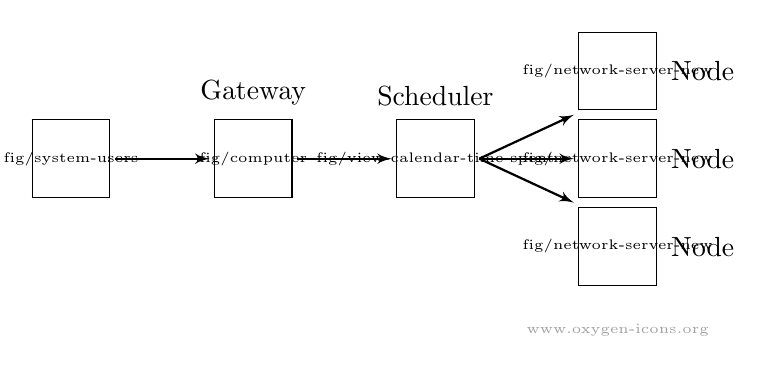
\begin{tikzpicture}[node distance=0cm and 1.2cm,auto]
\pgfdeclareimage[width=1cm]{user}{fig/system-users}
\pgfdeclareimage[width=1cm]{gateway}{fig/computer}
\pgfdeclareimage[width=1cm]{scheduler}{fig/view-calendar-time-spent}
\pgfdeclareimage[width=1cm]{node}{fig/network-server-new}
\pgfdeclareimage[width=0.5cm]{jobfile}{fig/document-open-recent}
\tikzstyle{line} = [draw,thick, -latex']
\tikzstyle{box} = [rectangle, minimum width=1.1cm, minimum height=1.1cm]
\tikzstyle{bg} = [rectangle]

\node (user) [box] {\pgfbox[center,center]{\pgfuseimage{user}}};
\node (gateway) [box] [right=of user, label=above:Gateway] {\pgfbox[center,center]{\pgfuseimage{gateway}}};
\node (scheduler) [box] [right=of gateway, label=above:Scheduler] {\pgfbox[center,center]{\pgfuseimage{scheduler}}};
\node (node2) [box] [right=of scheduler, label=right:Node] {\pgfbox[center,center]{\pgfuseimage{node}}};
\node (node1) [box] [above=of node2, label=right:Node] {\pgfbox[center,center]{\pgfuseimage{node}}};
\node (node3) [box] [below=of node2, label=right:Node] {\pgfbox[center,center]{\pgfuseimage{node}}};

\draw [line] (user.east) to (gateway.west);
\draw [line] (gateway.east) to (scheduler.west);
\draw [line] (scheduler.east) to (node1.south west);
\draw [line] (scheduler.east) to (node2.west);
\draw [line] (scheduler.east) to (node3.north west);

\node [rectangle, font=\tiny,color=gray] at ([yshift=-0.5cm]node3.south) {www.oxygen-icons.org};
\end{tikzpicture}
\end{adjustbox}
\end{center}
\begin{itemize}
\item User log onto the gateway server (master or head node)
\item Network of multiple computing nodes, managed by the scheduler
\item Scheduler orchestrates the computation and organizes queues to fairly distribute compuation times among users
\item Nodes either share a file system or a some form of file staging
\end{itemize}
\end{vbframe}

%\begin{vbframe}{Available resources for statisticians in Munich}
%\begin{blocki}{Leibniz Rechenzentrum (lrz): SLURM}
%\item $13936$ cores with peak performance of $479$ TFlop/s
%\item Mixed shared and distributed memory
%\item Flexible usage due to various available memory sizes
%\item Serial and parallel job processing
%\item Documentation: \url{lrz.de/services/compute/linux-cluster/}
%\end{blocki}

% \framebreak
%
% \begin{blocki}{University: LIDOng}
% \item Linux HPC cluster of the university
% \item Runs MAUI / TORQUE
% \item More than 3500 cores / 7 TB RAM
% \item Linpack peak: 23 TFlop/s
% \item Have used it successfully for several years now\\
% Many studies added up to years of (sequential) computation time.
% \end{blocki}
%\end{vbframe}

\begin{vbframe}{Manual working on a batch system}
\begin{itemize}
\item You have to specify
\begin{enumerate}[(a)]
\item Resource specifications (number CPUs, number of tasks, expected runtime and memory)
\item Which cluster use, e.g., serial, mpp2 or hugemem.
\item Command to execute (e.g. \code{R CMD BATCH <myscript.R>})
\end{enumerate}
\item Specs passed to CLI tools either directly as arguments or encoded in a shell script
\item Check status of jobs via CLI tools (e.g. \code{squeue})
\item Write script to collect results
\end{itemize}
\end{vbframe}

\begin{vbframe}{Usual workflow on a batch system}
\begin{itemize}
\item \textbf{Unroll} your \pkg{R} \textbf{loop(s)} so that your script computes a single iteration
\item Write a \textbf{script that writes \pkg{R} scripts} for each iteration setting the iteration counter(s) at the beginning
\item Write a \textbf{script that writes job description files} for each \pkg{R} script
\item Write a \textbf{script that submits} your job description files
\item \textbf{Crawl} through file system checking for existence of results or log files
\item Write a \textbf{script that combines} your scattered result files
\end{itemize}

\begin{itemize}
\item Found a bug in your code? Write a \textbf{script that kills} all running jobs, fix the bug, submit everything again
\item Some jobs have hit the wall time? Write a \textbf{script that finds} out which jobs you need to resubmit with weaker constraints
\item Want to try your model on another data set or using other parameters? Eventually \textbf{start from scratch}, it might get ugly
\end{itemize}
\end{vbframe}





% \begin{vbframe}{Synchronous vs. asynchronous computation}
% But we already know how snowfall works, why not simply do ...
% <<sf1, eval=FALSE, tidy=FALSE, cache=TRUE>>=
%   job.pbs
%   PBS -N my_parallel_job
%   ...
%   PBS -l nodes=100,walltime=5000,vmem=1024MB
%   R CMD BATCH job.R
%
%   job.R
%   sfInit(parallel = TRUE, type = "MPI", cpus = 100)
%   ys = sfLapply(xs, mySlaveFun)
%   sfStop()
%   @
%   \begin{itemize}
% \item You are now basically circumventing the scheduler
% \item How long are you willing to wait in queue? Infinitely?
% \item What if some jobs crash?
% \item What if you later want to add jobs?
% \item \textbf{One independent, embarrassingly parallel job should be submitted as such!}
% \end{itemize}
% \end{vbframe}

\begin{vbframe}{Conclusions and further remarks}
\begin{description}[12]
\item[\bf\color{checkgreen}+] They are pretty fast!
  \item[\bf\color{checkgreen}+] Many statistical tasks are embarrassingly parallel
\item[\bf\color{errorred}-] Job description files needed
\item[\bf\color{errorred}-] We cannot control when jobs are started.
\item[\bf\color{errorred}-] Jobs cannot really communicate, except by writing stuff on disk
(or we have to allocate multiple cores and use something like MPI)
\item[\bf\color{errorred}-] Requesting many nodes at once increases time spend in queue
\item[\bf\color{errorred}-] Auxiliary scripts to create files and submit jobs necessary
\item[\bf\color{errorred}-] Functions to collect results can get complicated and lengthy
\item[\bf\color{errorred}-] If some jobs fail (e.g, singularities), debugging is awful
\end{description}
\end{vbframe}


%%%%%%%%%%%%%%%%%%%%%%%%%%%%%%%%%%%%%%%%%%%%%%%%%%%%%%%%%%%%%%%%%%%%%%%%%%%%%%%%%%%%%%%%%%%%%%%%%%%
\section{The batchtools Package}
%%%%%%%%%%%%%%%%%%%%%%%%%%%%%%%%%%%%%%%%%%%%%%%%%%%%%%%%%%%%%%%%%%%%%%%%%%%%%%%%%%%%%%%%%%%%%%%%%%%

\begin{vbframe}{Packages}
\begin{blocki}{batchtools}
\item Basic infrastructure to communicate with a high performance cluster
\item Tailored around Map-Reduce paradigm
\item Can be incorporated into other packages
\item Supported via \pkg{parallelMap} and \code{BiocParallel}
\item Additional abstraction for \enquote{applying algorithms on problems}
\item Assists the user in conducting comprehensive computer experiments
\item Successor package (and combination) of \pkg{BatchJobs} and \pkg{BatchExperiments}.
\end{blocki}
\end{vbframe}


\begin{vbframe}{batchtools -- Features}
\begin{itemize}
\item Basic infrastructure to communicate with batch systems from within \pkg{R}
\item Complete control over the batch system from within \pkg{R}: submit, supervise, kill
\item Persistent state of computation for experiments
\item \pkg{R} code independent from the underlying batch system
\item Reproducibility in distributed environments, even if the architecture changes
\item Convenient result collection capabilities
\item Debugging tools
\end{itemize}
\end{vbframe}


\begin{vbframe}{Supported Systems}
Real batch systems:
  \begin{itemize}
\item Torque/PBS based systems
\item Sun Grid Engine / Oracle Grid Engine
\item Load Sharing Facility (LSF)
\item SLURM
\item DockerSwarm
\end{itemize}
\vfill
Other modes:
  \begin{itemize}
\item Interactive: Jobs executed in current interactive \pkg{R} session
\item Multicore: local multicore execution with spawned processes
\item SSH: distributed computing on loosely connected machines which are accessible via SSH (makeshift cluster)
\end{itemize}
\end{vbframe}


\begin{vbframe}{Links and references}
\begin{itemize}
\item {\large \url{https://github.com/mllg/batchtools}}
\begin{itemize}
\item Installation infos
\item R documentation
\item Vignettes
\item Issue tracker
\item Recent development version in git
\end{itemize}
\item Paper:\\
M Lang, B Bischl, D Surmann - The Journal of Open Source Software, 2017:\\
\textit{\enquote{batchtools: Tools for R to work on batch systems}}\\
Available on project page
  \end{itemize}
\end{vbframe}

\begin{vbframe}{(1) Create a registry}
\begin{itemize}
\item Object used to access and exchange informations: file paths, job parameters, computational events, \ldots
\item All information is stored in a single, portable directory
\item Initialization of a new registry:
\begin{knitrout}\scriptsize
\definecolor{shadecolor}{rgb}{0.969, 0.969, 0.969}\color{fgcolor}\begin{kframe}
\begin{alltt}
\hlstd{> }\hlkwd{library}\hlstd{(batchtools)}
\hlstd{> }\hlstd{reg} \hlkwb{=} \hlkwd{makeRegistry}\hlstd{(}
\hlstd{+ }\hlkwc{file.dir} \hlstd{=} \hlstr{"~/project"}\hlstd{,}          \hlcom{# accessible on all nodes}
\hlstd{+ }\hlkwc{seed} \hlstd{=} \hlnum{1}                         \hlcom{# initial seed for first job}
\hlstd{+ }\hlstd{)}
\end{alltt}
\end{kframe}
\end{knitrout}
\item \texttt{loadRegistry(dir)} to resume working with an existing registry
\end{itemize}
\end{vbframe}

%FIXME: where is extra-tex/overview???
%\begin{vbframe}[c]
% \begin{adjustbox}{width={1\textwidth}}
% \begin{tikzpicture}[auto]
%    \tikzstyle{box} = [rectangle, drop shadow, draw=black, fill=white, thick, minimum width=4cm, rounded corners, align=center,font=\ttfamily\large]
  \tikzstyle{chead} = [font=\large\bfseries]
  \tikzstyle{rhead} = [chead,align=left, minimum width=4cm]
  \tikzstyle{bg} = [rectangle, fill=gray!10, inner sep=0.2cm, rounded corners=5mm]
  \tikzstyle{hl} = [rectangle, draw=red, inner sep=0.2cm, rounded corners=5mm]

  \matrix [row sep=10mm, column sep=5mm] (mat) {
    \node (chead0) [minimum width=4cm] {}; \pgfmatrixnextcell
    \node (chead1) [chead] {BatchJobs' functions}; \pgfmatrixnextcell
    \node (chead2) [chead] {Common functions}; \pgfmatrixnextcell
    \node (chead3) [chead] {BatchExperiments' functions}; \\

    \node (registry0) [rhead] {(1) Create Registry}; \pgfmatrixnextcell
    \node (registry1) [box] {makeRegistry}; \pgfmatrixnextcell
    \node (registry2) {}; \pgfmatrixnextcell
    \node (registry3) [box] {makeExperimentRegistry}; \\

    \node (define0) [rhead] {(2) Define Jobs}; \pgfmatrixnextcell
    \node (define1) [box] {batchMap \\ batchReduce \\ batchExpandGrid}; \pgfmatrixnextcell
    \node (define2) [box] {batchMapResults \\ batchReduceResults}; \pgfmatrixnextcell
    \node (define3) [box] {addProblem \\ addAlgorithm \\ makeDesign \\ addExperiments}; \\

    \node (subsetting0) [rhead] {(3) Subset Jobs}; \pgfmatrixnextcell
    \node (subsetting1) [box] {findJobs}; \pgfmatrixnextcell
    \node (subsetting2) [box] {findDone\\ findErrors \\\ldots}; \pgfmatrixnextcell
    \node (subsetting3) [box] {findExperiments}; \\

    \node (submit0) [rhead] {(4) Submit Jobs}; \pgfmatrixnextcell
    \node (submit1) {}; \pgfmatrixnextcell
    \node (submit2) [box] {submitJobs}; \pgfmatrixnextcell
    \node (submit3) {}; \\

    \node (status0) [rhead] {(5) Status \& Debugging}; \pgfmatrixnextcell
    \node (status1) {}; \pgfmatrixnextcell
    \node (status2) [box] {showStatus \\ testJob \\ showLog}; \pgfmatrixnextcell
    \node (status3) [box] {summarizeExperiments}; \\

    \node (collect0) [rhead] {(6) Collect Results}; \pgfmatrixnextcell
    \node (collect1) {}; \pgfmatrixnextcell
    \node (collect2) [box] {loadResult[s] \\ reduceResults \\ filterResults \\ reduceResults[AggrType]}; \pgfmatrixnextcell
    \node (collect3) [box] {reduceResultsExperiments}; \\
  };
  \begin{pgfonlayer}{background}
    \node [bg, fit=(chead0) (collect0)] {};
    \node [bg, fit=(chead0) (chead3)] {};
  \end{pgfonlayer}

% \node [hl, fit=(define0) (define1) (define2)] {};
%\end{tikzpicture}
%\end{adjustbox}
%\end{vbframe}

\begin{vbframe}{(2) Define Jobs}
\begin{blocki}{\texttt{batchMap}}
\item Like \texttt{lapply} or \texttt{mapply}
\item $(x_1, x_2) \times (y_1, y_2) \rightarrow \left( f(x_1, y_1), f(x_2, y_2) \right)$
\item $10$~Jobs to calculate $1+9$, $2+8$, \ldots, $9+1$
\begin{knitrout}\scriptsize
\definecolor{shadecolor}{rgb}{0.969, 0.969, 0.969}\color{fgcolor}\begin{kframe}
\begin{alltt}
\hlstd{> }\hlstd{map} \hlkwb{=} \hlkwa{function}\hlstd{(}\hlkwc{i}\hlstd{,} \hlkwc{j}\hlstd{)  i} \hlopt{+}\hlstd{j}
\hlstd{> }\hlstd{ids} \hlkwb{=} \hlkwd{batchMap}\hlstd{(}\hlkwc{fun} \hlstd{= map,} \hlkwc{i} \hlstd{=} \hlnum{1}\hlopt{:}\hlnum{9}\hlstd{,} \hlkwc{j} \hlstd{=} \hlnum{9}\hlopt{:}\hlnum{1}\hlstd{,} \hlkwc{reg} \hlstd{= reg)}
\end{alltt}
\end{kframe}
\end{knitrout}
\item Stores function on file system
\item Creates jobs as rows in a \pkg{data.table}
\item Parameters also serialized into the \pkg{data.table} for fast access
\item All jobs get unique positive integers as IDs
\item \texttt{reg =} can be omitted in most cases. See \texttt{getDefaultRegistry}.
\end{blocki}
\end{vbframe}


%FIXME: where is extra-tex/overview???
%\begin{vbframe}[c]
%  \begin{adjustbox}{width={1\textwidth}}
%  \begin{tikzpicture}[auto]
%      \tikzstyle{box} = [rectangle, drop shadow, draw=black, fill=white, thick, minimum width=4cm, rounded corners, align=center,font=\ttfamily\large]
  \tikzstyle{chead} = [font=\large\bfseries]
  \tikzstyle{rhead} = [chead,align=left, minimum width=4cm]
  \tikzstyle{bg} = [rectangle, fill=gray!10, inner sep=0.2cm, rounded corners=5mm]
  \tikzstyle{hl} = [rectangle, draw=red, inner sep=0.2cm, rounded corners=5mm]

  \matrix [row sep=10mm, column sep=5mm] (mat) {
    \node (chead0) [minimum width=4cm] {}; \pgfmatrixnextcell
    \node (chead1) [chead] {BatchJobs' functions}; \pgfmatrixnextcell
    \node (chead2) [chead] {Common functions}; \pgfmatrixnextcell
    \node (chead3) [chead] {BatchExperiments' functions}; \\

    \node (registry0) [rhead] {(1) Create Registry}; \pgfmatrixnextcell
    \node (registry1) [box] {makeRegistry}; \pgfmatrixnextcell
    \node (registry2) {}; \pgfmatrixnextcell
    \node (registry3) [box] {makeExperimentRegistry}; \\

    \node (define0) [rhead] {(2) Define Jobs}; \pgfmatrixnextcell
    \node (define1) [box] {batchMap \\ batchReduce \\ batchExpandGrid}; \pgfmatrixnextcell
    \node (define2) [box] {batchMapResults \\ batchReduceResults}; \pgfmatrixnextcell
    \node (define3) [box] {addProblem \\ addAlgorithm \\ makeDesign \\ addExperiments}; \\

    \node (subsetting0) [rhead] {(3) Subset Jobs}; \pgfmatrixnextcell
    \node (subsetting1) [box] {findJobs}; \pgfmatrixnextcell
    \node (subsetting2) [box] {findDone\\ findErrors \\\ldots}; \pgfmatrixnextcell
    \node (subsetting3) [box] {findExperiments}; \\

    \node (submit0) [rhead] {(4) Submit Jobs}; \pgfmatrixnextcell
    \node (submit1) {}; \pgfmatrixnextcell
    \node (submit2) [box] {submitJobs}; \pgfmatrixnextcell
    \node (submit3) {}; \\

    \node (status0) [rhead] {(5) Status \& Debugging}; \pgfmatrixnextcell
    \node (status1) {}; \pgfmatrixnextcell
    \node (status2) [box] {showStatus \\ testJob \\ showLog}; \pgfmatrixnextcell
    \node (status3) [box] {summarizeExperiments}; \\

    \node (collect0) [rhead] {(6) Collect Results}; \pgfmatrixnextcell
    \node (collect1) {}; \pgfmatrixnextcell
    \node (collect2) [box] {loadResult[s] \\ reduceResults \\ filterResults \\ reduceResults[AggrType]}; \pgfmatrixnextcell
    \node (collect3) [box] {reduceResultsExperiments}; \\
  };
  \begin{pgfonlayer}{background}
    \node [bg, fit=(chead0) (collect0)] {};
    \node [bg, fit=(chead0) (chead3)] {};
  \end{pgfonlayer}

%    \node [hl, fit=(subsetting0) (subsetting1) (subsetting2)] {};
%  \end{tikzpicture}
%\end{adjustbox}
%\end{vbframe}

\begin{vbframe}{(3) Subset Jobs}
\begin{itemize}
\item Query job IDs by computational status: \texttt{find*} functions \\\texttt{findSubmitted}, \texttt{findRunning}, \texttt{findDone}, \ldots
\item Query job IDs by parameters: \texttt{findJobs(pars)}
\begin{knitrout}\scriptsize
\definecolor{shadecolor}{rgb}{0.969, 0.969, 0.969}\color{fgcolor}\begin{kframe}
\begin{alltt}
\hlstd{> }\hlkwd{findJobs}\hlstd{(j}\hlopt{==}\hlnum{1}\hlstd{)}
\hlstd{> }\hlkwd{findNotSubmitted}\hlstd{()}
\hlstd{> }\hlkwd{findDone}\hlstd{()}
\end{alltt}
\end{kframe}
\end{knitrout}
  \item Set operations on ID \pkg{data.tables}: \texttt{merge}
\item \pkg{data.table} of IDs can be passed to basically all functions interacting with the batch system
\end{itemize}
\end{vbframe}

%FIXME: Couldnt find extra-tex/overview in the repo.....
%\begin{vbframe}[c]
%  \begin{adjustbox}{width={1\textwidth}}
%  \begin{tikzpicture}[auto]
%      \tikzstyle{box} = [rectangle, drop shadow, draw=black, fill=white, thick, minimum width=4cm, rounded corners, align=center,font=\ttfamily\large]
  \tikzstyle{chead} = [font=\large\bfseries]
  \tikzstyle{rhead} = [chead,align=left, minimum width=4cm]
  \tikzstyle{bg} = [rectangle, fill=gray!10, inner sep=0.2cm, rounded corners=5mm]
  \tikzstyle{hl} = [rectangle, draw=red, inner sep=0.2cm, rounded corners=5mm]

  \matrix [row sep=10mm, column sep=5mm] (mat) {
    \node (chead0) [minimum width=4cm] {}; \pgfmatrixnextcell
    \node (chead1) [chead] {BatchJobs' functions}; \pgfmatrixnextcell
    \node (chead2) [chead] {Common functions}; \pgfmatrixnextcell
    \node (chead3) [chead] {BatchExperiments' functions}; \\

    \node (registry0) [rhead] {(1) Create Registry}; \pgfmatrixnextcell
    \node (registry1) [box] {makeRegistry}; \pgfmatrixnextcell
    \node (registry2) {}; \pgfmatrixnextcell
    \node (registry3) [box] {makeExperimentRegistry}; \\

    \node (define0) [rhead] {(2) Define Jobs}; \pgfmatrixnextcell
    \node (define1) [box] {batchMap \\ batchReduce \\ batchExpandGrid}; \pgfmatrixnextcell
    \node (define2) [box] {batchMapResults \\ batchReduceResults}; \pgfmatrixnextcell
    \node (define3) [box] {addProblem \\ addAlgorithm \\ makeDesign \\ addExperiments}; \\

    \node (subsetting0) [rhead] {(3) Subset Jobs}; \pgfmatrixnextcell
    \node (subsetting1) [box] {findJobs}; \pgfmatrixnextcell
    \node (subsetting2) [box] {findDone\\ findErrors \\\ldots}; \pgfmatrixnextcell
    \node (subsetting3) [box] {findExperiments}; \\

    \node (submit0) [rhead] {(4) Submit Jobs}; \pgfmatrixnextcell
    \node (submit1) {}; \pgfmatrixnextcell
    \node (submit2) [box] {submitJobs}; \pgfmatrixnextcell
    \node (submit3) {}; \\

    \node (status0) [rhead] {(5) Status \& Debugging}; \pgfmatrixnextcell
    \node (status1) {}; \pgfmatrixnextcell
    \node (status2) [box] {showStatus \\ testJob \\ showLog}; \pgfmatrixnextcell
    \node (status3) [box] {summarizeExperiments}; \\

    \node (collect0) [rhead] {(6) Collect Results}; \pgfmatrixnextcell
    \node (collect1) {}; \pgfmatrixnextcell
    \node (collect2) [box] {loadResult[s] \\ reduceResults \\ filterResults \\ reduceResults[AggrType]}; \pgfmatrixnextcell
    \node (collect3) [box] {reduceResultsExperiments}; \\
  };
  \begin{pgfonlayer}{background}
    \node [bg, fit=(chead0) (collect0)] {};
    \node [bg, fit=(chead0) (chead3)] {};
  \end{pgfonlayer}

%    \node [hl, fit=(submit0) (submit1) (submit2)] {};
%  \end{tikzpicture}
%\end{adjustbox}
%\end{vbframe}

\begin{vbframe}{(4) Submit Jobs}
\begin{blocki}{\texttt{submitJobs}}
\item Creates \pkg{R} script files and job description files on the fly
\item Resources can be provided as named list
\begin{knitrout}\scriptsize
\definecolor{shadecolor}{rgb}{0.969, 0.969, 0.969}\color{fgcolor}\begin{kframe}
\begin{alltt}
\hlstd{> }\hlcom{# 1 hour maximal execution time, about 2 GB of RAM}
\hlstd{> }\hlstd{res} \hlkwb{=} \hlkwd{list}\hlstd{(}\hlkwc{walltime} \hlstd{=} \hlnum{60}\hlopt{*}\hlnum{60}\hlstd{,} \hlkwc{memory} \hlstd{=} \hlnum{2000}\hlstd{)}
\hlstd{> }
\hlstd{> }\hlcom{# ... and submit}
\hlstd{> }\hlkwd{submitJobs}\hlstd{(}\hlkwc{resources} \hlstd{= res)}
\end{alltt}
\end{kframe}
\end{knitrout}
  \item Submits all jobs per default
\item Subsets of jobs can be providing as \pkg{data.table} or \texttt{vector}
\begin{knitrout}\scriptsize
\definecolor{shadecolor}{rgb}{0.969, 0.969, 0.969}\color{fgcolor}\begin{kframe}
\begin{alltt}
\hlstd{> }  \hlkwd{submitJobs}\hlstd{(}\hlkwc{ids} \hlstd{=} \hlnum{1}\hlopt{:}\hlnum{5}\hlstd{,} \hlkwc{ressources} \hlstd{= res)}
\end{alltt}
\end{kframe}
\end{knitrout}
  \end{blocki}
\end{vbframe}

%FIXME: Couldnt find extra-tex/overview in the repo.....
%\begin{vbframe}[c]
%  \begin{adjustbox}{width={1\textwidth}}
%  \begin{tikzpicture}[auto]
%      \tikzstyle{box} = [rectangle, drop shadow, draw=black, fill=white, thick, minimum width=4cm, rounded corners, align=center,font=\ttfamily\large]
  \tikzstyle{chead} = [font=\large\bfseries]
  \tikzstyle{rhead} = [chead,align=left, minimum width=4cm]
  \tikzstyle{bg} = [rectangle, fill=gray!10, inner sep=0.2cm, rounded corners=5mm]
  \tikzstyle{hl} = [rectangle, draw=red, inner sep=0.2cm, rounded corners=5mm]

  \matrix [row sep=10mm, column sep=5mm] (mat) {
    \node (chead0) [minimum width=4cm] {}; \pgfmatrixnextcell
    \node (chead1) [chead] {BatchJobs' functions}; \pgfmatrixnextcell
    \node (chead2) [chead] {Common functions}; \pgfmatrixnextcell
    \node (chead3) [chead] {BatchExperiments' functions}; \\

    \node (registry0) [rhead] {(1) Create Registry}; \pgfmatrixnextcell
    \node (registry1) [box] {makeRegistry}; \pgfmatrixnextcell
    \node (registry2) {}; \pgfmatrixnextcell
    \node (registry3) [box] {makeExperimentRegistry}; \\

    \node (define0) [rhead] {(2) Define Jobs}; \pgfmatrixnextcell
    \node (define1) [box] {batchMap \\ batchReduce \\ batchExpandGrid}; \pgfmatrixnextcell
    \node (define2) [box] {batchMapResults \\ batchReduceResults}; \pgfmatrixnextcell
    \node (define3) [box] {addProblem \\ addAlgorithm \\ makeDesign \\ addExperiments}; \\

    \node (subsetting0) [rhead] {(3) Subset Jobs}; \pgfmatrixnextcell
    \node (subsetting1) [box] {findJobs}; \pgfmatrixnextcell
    \node (subsetting2) [box] {findDone\\ findErrors \\\ldots}; \pgfmatrixnextcell
    \node (subsetting3) [box] {findExperiments}; \\

    \node (submit0) [rhead] {(4) Submit Jobs}; \pgfmatrixnextcell
    \node (submit1) {}; \pgfmatrixnextcell
    \node (submit2) [box] {submitJobs}; \pgfmatrixnextcell
    \node (submit3) {}; \\

    \node (status0) [rhead] {(5) Status \& Debugging}; \pgfmatrixnextcell
    \node (status1) {}; \pgfmatrixnextcell
    \node (status2) [box] {showStatus \\ testJob \\ showLog}; \pgfmatrixnextcell
    \node (status3) [box] {summarizeExperiments}; \\

    \node (collect0) [rhead] {(6) Collect Results}; \pgfmatrixnextcell
    \node (collect1) {}; \pgfmatrixnextcell
    \node (collect2) [box] {loadResult[s] \\ reduceResults \\ filterResults \\ reduceResults[AggrType]}; \pgfmatrixnextcell
    \node (collect3) [box] {reduceResultsExperiments}; \\
  };
  \begin{pgfonlayer}{background}
    \node [bg, fit=(chead0) (collect0)] {};
    \node [bg, fit=(chead0) (chead3)] {};
  \end{pgfonlayer}

%    \node [hl, fit=(status0) (status1) (status2)] {};
%  \end{tikzpicture}
%\end{adjustbox}
%\end{vbframe}

\begin{vbframe}{(5) Supervise and debug}
\begin{itemize}
\item Quick overview of what is going on: \texttt{getStatus()}
\begin{verbatim}
Status for jobs:  10
Submitted:        10 (100.0%)
Started:          10 (100.0%)
Errors:            0 (  0.0%)
Running:           2 ( 20.0%)
Expired:           0 (  0.0%)
Done:              8 ( 80.0%)
Time: min=1.50s avg=5.20s max=8.80s
\end{verbatim}
\item Display log files with a customizable pager (less, vi, ...): \\ \texttt{showLog(findErrors()[1])}
\item You can also \texttt{grepLogs(pattern)}
\item Found a bug? \texttt{killJobs(findRunning())}
\item Run a job in the current \pkg{R} session: \texttt{testJob(id)}
\end{itemize}
\end{vbframe}

%FIXME: Couldnt find extra-tex/overview in the repo.....
%\begin{vbframe}[c]
%  \begin{adjustbox}{width={1\textwidth}}
%  \begin{tikzpicture}[auto]
%      \tikzstyle{box} = [rectangle, drop shadow, draw=black, fill=white, thick, minimum width=4cm, rounded corners, align=center,font=\ttfamily\large]
  \tikzstyle{chead} = [font=\large\bfseries]
  \tikzstyle{rhead} = [chead,align=left, minimum width=4cm]
  \tikzstyle{bg} = [rectangle, fill=gray!10, inner sep=0.2cm, rounded corners=5mm]
  \tikzstyle{hl} = [rectangle, draw=red, inner sep=0.2cm, rounded corners=5mm]

  \matrix [row sep=10mm, column sep=5mm] (mat) {
    \node (chead0) [minimum width=4cm] {}; \pgfmatrixnextcell
    \node (chead1) [chead] {BatchJobs' functions}; \pgfmatrixnextcell
    \node (chead2) [chead] {Common functions}; \pgfmatrixnextcell
    \node (chead3) [chead] {BatchExperiments' functions}; \\

    \node (registry0) [rhead] {(1) Create Registry}; \pgfmatrixnextcell
    \node (registry1) [box] {makeRegistry}; \pgfmatrixnextcell
    \node (registry2) {}; \pgfmatrixnextcell
    \node (registry3) [box] {makeExperimentRegistry}; \\

    \node (define0) [rhead] {(2) Define Jobs}; \pgfmatrixnextcell
    \node (define1) [box] {batchMap \\ batchReduce \\ batchExpandGrid}; \pgfmatrixnextcell
    \node (define2) [box] {batchMapResults \\ batchReduceResults}; \pgfmatrixnextcell
    \node (define3) [box] {addProblem \\ addAlgorithm \\ makeDesign \\ addExperiments}; \\

    \node (subsetting0) [rhead] {(3) Subset Jobs}; \pgfmatrixnextcell
    \node (subsetting1) [box] {findJobs}; \pgfmatrixnextcell
    \node (subsetting2) [box] {findDone\\ findErrors \\\ldots}; \pgfmatrixnextcell
    \node (subsetting3) [box] {findExperiments}; \\

    \node (submit0) [rhead] {(4) Submit Jobs}; \pgfmatrixnextcell
    \node (submit1) {}; \pgfmatrixnextcell
    \node (submit2) [box] {submitJobs}; \pgfmatrixnextcell
    \node (submit3) {}; \\

    \node (status0) [rhead] {(5) Status \& Debugging}; \pgfmatrixnextcell
    \node (status1) {}; \pgfmatrixnextcell
    \node (status2) [box] {showStatus \\ testJob \\ showLog}; \pgfmatrixnextcell
    \node (status3) [box] {summarizeExperiments}; \\

    \node (collect0) [rhead] {(6) Collect Results}; \pgfmatrixnextcell
    \node (collect1) {}; \pgfmatrixnextcell
    \node (collect2) [box] {loadResult[s] \\ reduceResults \\ filterResults \\ reduceResults[AggrType]}; \pgfmatrixnextcell
    \node (collect3) [box] {reduceResultsExperiments}; \\
  };
  \begin{pgfonlayer}{background}
    \node [bg, fit=(chead0) (collect0)] {};
    \node [bg, fit=(chead0) (chead3)] {};
  \end{pgfonlayer}

%    \node [hl, fit=(collect0) (collect1) (collect2)] {};
%  \end{tikzpicture}
%\end{adjustbox}
%\end{vbframe}

\begin{vbframe}{(6) Collect results}

\begin{block}{Reduce}
\begin{knitrout}\scriptsize
\definecolor{shadecolor}{rgb}{0.969, 0.969, 0.969}\color{fgcolor}\begin{kframe}
\begin{alltt}
\hlstd{> }\hlcom{# combine in numeric vector}
\hlstd{> }\hlkwd{reduceResults}\hlstd{(}\hlkwc{ids} \hlstd{=} \hlkwd{findDone}\hlstd{(),} \hlkwc{init} \hlstd{=} \hlkwd{numeric}\hlstd{(}\hlnum{0}\hlstd{),}
\hlstd{+ }              \hlkwc{fun} \hlstd{=} \hlkwa{function}\hlstd{(}\hlkwc{aggr}\hlstd{,} \hlkwc{job}\hlstd{,} \hlkwc{res}\hlstd{)} \hlkwd{c}\hlstd{(aggr, res))}
\end{alltt}
\end{kframe}
\end{knitrout}
\begin{itemize}
\item Convenience wrappers around \texttt{reduceResults}: \texttt{reduceResults[DataTable|List]}
\item {Simple loading}
\begin{knitrout}\scriptsize
\definecolor{shadecolor}{rgb}{0.969, 0.969, 0.969}\color{fgcolor}\begin{kframe}
\begin{alltt}
\hlstd{> }\hlkwd{loadResult}\hlstd{(}\hlkwc{id} \hlstd{=} \hlnum{1}\hlstd{)}
\end{alltt}
\end{kframe}
\end{knitrout}
\end{itemize}
\end{block}

\end{vbframe}

% \begin{vbframe}
% \centering\Large
% {Coffee / Demo}
% \end{vbframe}
%
% \begin{vbframe}{Seeding}
% \begin{itemize}
% \item Every job has a unique seed
% \item Registry stores initial seed $x_0$, all job seeds are defined as $x_0$ + ID
% \item In some rare cases you need to manually change seeds, therefore all seeds are stored in DB
% \item Jobs become reproducible, even on another site
% \item But note all other ugly problems due to changes in hardware, software, compilers, versions, \ldots
% \end{itemize}
% \end{vbframe}
%
\begin{vbframe}{Configuration again}
\texttt{.batchtools.conf.R}
\begin{knitrout}\scriptsize
\definecolor{shadecolor}{rgb}{0.969, 0.969, 0.969}\color{fgcolor}\begin{kframe}
\begin{alltt}
\hlstd{> }\hlstd{cluster.functions} \hlkwb{=} \hlkwd{makeClusterFunctionsSlurm}\hlstd{(}\hlstr{"~/slurm_lmulrz.tmpl"}\hlstd{,} \hlkwc{array.jobs} \hlstd{=} \hlnum{FALSE}\hlstd{)}
\hlstd{> }\hlstd{default.resources} \hlkwb{=} \hlkwd{list}\hlstd{(}\hlkwc{walltime} \hlstd{=} \hlnum{300L}\hlstd{,} \hlkwc{memory} \hlstd{=} \hlnum{512L}\hlstd{,} \hlkwc{ntasks} \hlstd{=} \hlnum{1L}\hlstd{,} \hlkwc{ncpus} \hlstd{=} \hlnum{1L}\hlstd{,}
\hlstd{+ }  \hlkwc{nodes} \hlstd{=} \hlnum{1L}\hlstd{,} \hlkwc{clusters} \hlstd{=} \hlstr{"serial"}\hlstd{)}
\hlstd{> }
\hlstd{> }\hlstd{max.concurrent.jobs} \hlkwb{=} \hlnum{1000L}
\end{alltt}
\end{kframe}
\end{knitrout}
\end{vbframe}

\begin{vbframe}{Demo of basic usage}
\begin{knitrout}\scriptsize
\definecolor{shadecolor}{rgb}{0.969, 0.969, 0.969}\color{fgcolor}\begin{kframe}
\begin{alltt}
\hlstd{> }\hlkwd{unlink}\hlstd{(}\hlstr{"~/project"}\hlstd{,} \hlkwc{recursive} \hlstd{=} \hlnum{TRUE}\hlstd{)}
\hlstd{> }
\hlstd{> }\hlkwd{library}\hlstd{(batchtools)}
\hlstd{> }\hlstd{reg} \hlkwb{=} \hlkwd{makeRegistry}\hlstd{(}
\hlstd{+ }  \hlkwc{file.dir} \hlstd{=} \hlstr{"~/project"}\hlstd{,}          \hlcom{# path to store everything}
\hlstd{+ }  \hlkwc{seed} \hlstd{=} \hlnum{1}                         \hlcom{# initial seed for first job}
\hlstd{+ }\hlstd{)}
\hlstd{> }
\hlstd{> }\hlstd{f} \hlkwb{=} \hlkwa{function}\hlstd{(}\hlkwc{i}\hlstd{,} \hlkwc{j}\hlstd{) i}\hlopt{+}\hlstd{j}
\hlstd{> }\hlstd{ids} \hlkwb{=} \hlkwd{batchMap}\hlstd{(}\hlkwc{fun} \hlstd{= f,} \hlkwc{i} \hlstd{=} \hlnum{1}\hlopt{:}\hlnum{9}\hlstd{,} \hlkwc{j} \hlstd{=} \hlnum{9}\hlopt{:}\hlnum{1}\hlstd{)}
\hlstd{> }
\hlstd{> }\hlkwd{findJobs}\hlstd{(}\hlkwc{expr} \hlstd{= j} \hlopt{==} \hlnum{1}\hlstd{)}
\hlstd{> }\hlkwd{findNotSubmitted}\hlstd{()}
\hlstd{> }\hlkwd{findDone}\hlstd{()}
\end{alltt}
\end{kframe}
\end{knitrout}


\begin{knitrout}\scriptsize
\definecolor{shadecolor}{rgb}{0.969, 0.969, 0.969}\color{fgcolor}\begin{kframe}
\begin{alltt}
\hlstd{> }\hlstd{resources} \hlkwb{=} \hlkwd{list}\hlstd{(}\hlkwc{walltime} \hlstd{=} \hlnum{5}\hlopt{*}\hlnum{60}\hlstd{,} \hlkwc{memory} \hlstd{=} \hlnum{512}\hlstd{)}
\hlstd{> }\hlkwd{submitJobs}\hlstd{(}\hlkwc{resources} \hlstd{= resources)}
\hlstd{> }
\hlstd{> }\hlkwd{getStatus}\hlstd{()}
\hlstd{> }\hlkwd{waitForJobs}\hlstd{()}
\hlstd{> }\hlkwd{getStatus}\hlstd{()}
\hlstd{> }
\hlstd{> }\hlcom{# a peek into the database}
\hlstd{> }\hlkwd{getJobTable}\hlstd{(}\hlnum{1}\hlopt{:}\hlnum{2}\hlstd{)}
\hlstd{> }
\hlstd{> }\hlcom{# get results}
\hlstd{> }\hlkwd{loadResult}\hlstd{(}\hlnum{1}\hlstd{)}
\hlstd{> }\hlkwd{reduceResultsList}\hlstd{()}
\hlstd{> }\hlkwd{getJobTable}\hlstd{()[}\hlkwd{reduceResultsDataTable}\hlstd{()]}
\end{alltt}
\end{kframe}
\end{knitrout}
\end{vbframe}


% \begin{vbframe}{Some nice extra stuff I missed to explain}
% \begin{itemize}
% \item Reducing in parallel (\code{batchReduceResults()})
% \item Parallel work on previous results (\code{batchMapResults()})
% \item SSH mode (combine loosely connected boxes to a makeshift cluster with rudimentary scheduler)
% \item Using multicore or MPI jobs inside of batch jobs
% \item Submitting extremely many jobs (or: how to write your own daemon)
% \end{itemize}
% \end{vbframe}
%
%
% %%%%%%%%%%%%%%%%%%%%%%%%%%%%%%%%%%%%%%%%%%%%%%%%%%%%%%%%%%%%%%%%%%%%%%%%%%%%%%%%%%%%%%%%%%%%%%%%%%%
% \section{parallelMap as frontend}
% %%%%%%%%%%%%%%%%%%%%%%%%%%%%%%%%%%%%%%%%%%%%%%%%%%%%%%%%%%%%%%%%%%%%%%%%%%%%%%%%%%%%%%%%%%%%%%%%%%%
% \begin{vbframe}{parallelMap as BatchJobs frontend}
% <<eval=FALSE>>=
% library(parallelMap)
% parallelStartBatchJobs(bj.resources = list(),
%                        storagedir = "~/project/bj-files/")
% res = parallelMap(function(x) x^2, 1:10)
% parallelStop()
% @
% \begin{itemize}
% \item \code{parallelStartBatchJobs()} creates registry in \code{storagedir}
% \item \code{parallelMap()} creates jobs, submits them and waits for their termination, i.e.
% \begin{enumerate}
% \item \code{batchMap()}
% \item \code{submitJobs()}
% \item \code{waitForJobs()}
% \end{enumerate}
% \item \code{parallelStop()} cleans up the registry dir
% \end{itemize}
% \end{vbframe}
%
% \begin{vbframe}
% \centering\Large
% {Demo}
% \end{vbframe}
%
% \begin{vbframe}
% \centering\Large
% {Demo on SLURM}
% \end{vbframe}
%
%
%
%
%
% %%%%%%%%%%%%%%%%%%%%%%%%%%%%%%%%%%%%%%%%%%%%%%%%%%%%%%%%%%%%%%%%%%%%%%%%%
% %%%%%%%%%%%%%%%%%%DAY 5%%%%%%%%%%%%%%%%%%%%%%%%%%%%%%%%%%%%%%%%%%%%%%%%%%
% %%%%%%%%%%%%%%%%%%%%%%%%%%%%%%%%%%%%%%%%%%%%%%%%%%%%%%%%%%%%%%%%%%%%%%%%%
%
% %%%%%%%%%%%%%%%%%%%%%%%%%%%%%%%%%%%%%%%%%%%%%%%%%%%%%%%%%%%%%%%%%%%%%%%%%%%%%%%%%%%%%%%%%%%%%%%%%%%
% \section{BatchJobs II}
% %%%%%%%%%%%%%%%%%%%%%%%%%%%%%%%%%%%%%%%%%%%%%%%%%%%%%%%%%%%%%%%%%%%%%%%%%%%%%%%%%%%%%%%%%%%%%%%%%%%
%
% \begin{vbframe}{}
% \centering\Large
% {Demo expandGrid}
% \end{vbframe}
%
% \begin{vbframe}{}
% \centering\Large
% {Demo batchMapResults}
% \end{vbframe}
%
% \begin{vbframe}{}
% \centering\Large
% {Demo on LIDO}
% \end{vbframe}
%
% \begin{vbframe}{}
% \centering\Large
% {Demo: tmux with many jobs}
% \end{vbframe}
%
% \begin{vbframe}{}
% \centering\Large
% {SSH Demo on AZURE}
% \end{vbframe}
%
%
% %%%%%%%%%%%%%%%%%%%%%%%%%%%%%%%%%%%%%%%%%%%%%%%%%%%%%%%%%%%%%%%%%%%%%%%%%%%%%%%%%%%%%%%%%%%%%%%%%%%%%%%%%%%%%%%%%%%%%%%
\section{Abstractions for computer experiments}
%%%%%%%%%%%%%%%%%%%%%%%%%%%%%%%%%%%%%%%%%%%%%%%%%%%%%%%%%%%%%%%%%%%%%%%%%%%%%%%%%%%%%%%%%%%%%%%%%%%%%%%%%%%%%%%%%%%%%%%

\begin{vbframe}{Experiments in batchtools}
\begin{itemize}
\item Intended as abstraction for typical statistical tasks:\\
\begin{center}\textbf{Applying algorithms on problems}\end{center}
\item More aimed at the end user
\item Convenient for simulation studies, comparison and benchmark experiments, sensitivity analysis, \ldots
\item Workflow differs only in job definition
\item Scenarios:
\begin{itemize}
\item Compare machine learning algorithms on many data sets
\item Compare one/many estimation procedure(s) on simulated data
\item Compare optimizers on objective functions
\item \ldots
\end{itemize}
\end{itemize}
\end{vbframe}


\begin{vbframe}{Abstraction of Computer Experiments}
\begin{adjustbox}{width={1\textwidth}}
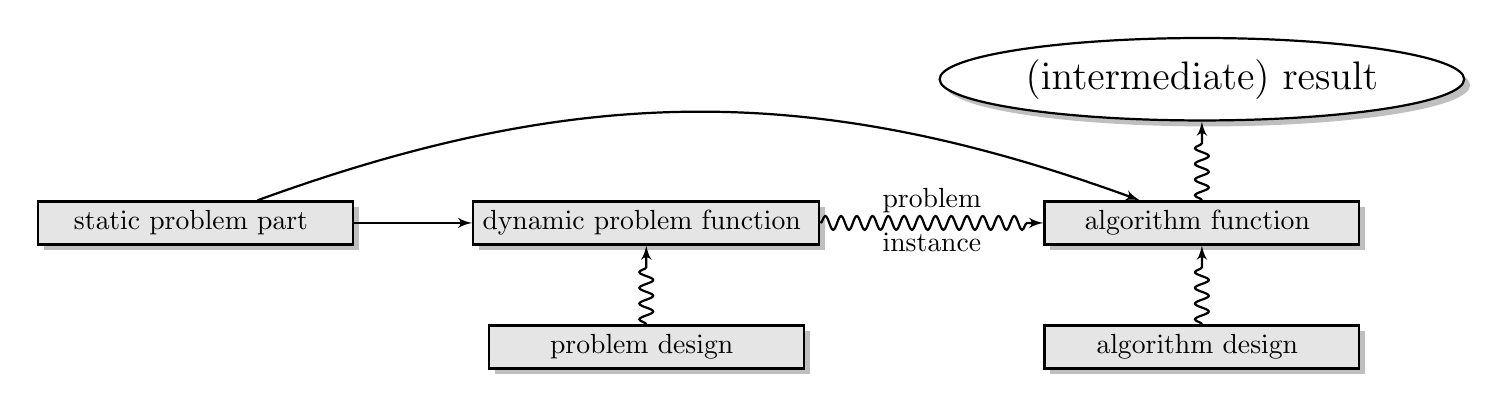
\begin{tikzpicture}[auto]
  % styles
  \tikzstyle{userinput}=[rectangle, drop shadow, draw=black, fill=black!10, thick, minimum width=4cm, align=center]

  \tikzstyle{internal}=[rectangle, drop shadow, draw=black, fill=white, thick, minimum width=4cm, rounded corners, align=center]
  \tikzstyle{result}=[ellipse, drop shadow, draw=black, fill=white, thick, align=center]
  \tikzstyle{line} = [draw, thick, -latex']
  \tikzstyle{sline} = [draw, thick, -latex',decorate, decoration={snake, segment length=2mm,post length=2mm}]

  \matrix [row sep=10mm, column sep=15mm] {
    % first row
    \node {}; &
    \node {}; &
    \node [result] (result) {\Large{(intermediate) result}}; \\

    % second row
    \node [userinput] (static_problem_part) {
        static problem part
    }; &
  \node [userinput] (dynamic_problem_part) {
          dynamic problem function
	}; &
	\node [userinput] (algorithm) {
        algorithm function
	}; \\

	% third row
	\node {}; &
    \node [userinput] (problem_design) {
        problem design
    }; &
	\node [userinput] (algorithm_design) {
        algorithm design
	}; \\
  };

  \draw [sline] (algorithm) to (result) ;
  \draw [line] (static_problem_part) to (dynamic_problem_part);
  \draw [sline] (dynamic_problem_part) to node {problem} node [swap] {instance} (algorithm) ;
  \draw [line] (static_problem_part) to [out=0, in=0, bend left=20] (algorithm);

  \draw [sline] (problem_design) to (dynamic_problem_part);
  \draw [sline] (algorithm_design) to (algorithm);
\end{tikzpicture}

\end{adjustbox}
\begin{itemize}
\item Problem definition split into static and dynamic part
\begin{itemize}
\item Static: immutable \pkg{R} objects: matrix, data frames, \ldots
\item Dynamic: Arbitrary \pkg{R} function: transformations of static part, extraction of data from external sources, \ldots
\end{itemize}
\item Parametrization through specifying experimental designs for both problems and algorithms
\item Each step automatically seeded, random seeds stored in a database
\end{itemize}
\end{vbframe}


\begin{vbframe}{Experiment definition steps}
\begin{enumerate}
\item Add problems to registry: \texttt{addProblem}
\begin{itemize}
\item Efficient storage: Separation of static (\texttt{data}) and dynamic (\texttt{instance}) problem parts.
\end{itemize}
\item Add algorithms to registry: \texttt{addAlgorithm}
\begin{itemize}
\item Problem instance gets passed to algorithm
\item Can be connected with an experimental design (function parameters)
\item Return value will be saved on the file system
\end{itemize}
\item Add experiments to registry: \texttt{addExperiments}
\begin{itemize}
\item Experiment: problem instance + algorithm + algorithm parameters
\item Job: Experiment + replication number
\end{itemize}
\end{enumerate}
\end{vbframe}


%\begin{vbframe}{A stupid example}
%<<eval=FALSE, size = "scriptsize">>=
%reg = makeExperimentRegistry("stupid")
%addProblem(name = "p1", data = 1, fun = function(data, job) runif(data))
%addAlgorithm(name = "a1",
%  fun = function(job, data, instance) 2 * instance)
%addAlgorithm(name = "a2",
%  fun = function(job, data, instance) data + instance)
%addExperiments(repls = 2)
%submitJobs()
%res = reduceResultsDataTable()
%getJobPars()[res]
%
%#   job.id problem algorithm        V1
%#1:      1      p1        a1 0.8617642
%#2:      2      p1        a1 0.9606042
%#3:      3      p1        a2 1.9529027
%#4:      4      p1        a2 1.5205857
%@
%
%
%  \end{vbframe}
%
%\begin{vbframe}{Classification example}
%\begin{itemize}
%\item Data frame is the static problem part
%\item Cross-validation function for index sets is dynamic problem part
%\item Fold number can be seen as a parameter of the problem
%\item Algorithms are the inducers, they return a cross-validated score
%\item Algorithms always have parameters (e.g. number of trees in a forest)
%\item Algorithm's results get automatically saved to the file system and can later be reduced
%\end{itemize}
%\end{vbframe}
%
%\begin{vbframe}{Demo classification}
%
%<<eval=FALSE>>=
%library(mlr)
%library(OpenML)
%library(batchtools)
%
%tasks = listOMLTasks(
%  number.of.missing.values = 0,
%  number.of.classes = 2,
%  number.of.features = c(4, 4),
%  number.of.instances = c(100, 200))
%@
%
%<<eval=FALSE>>=
%# create registry
%unlink("be_mlr_oml-files", recursive = TRUE)
%reg = makeExperimentRegistry("be_mlr_oml",
%  packages= c("mlr", "OpenML"))
%
%# generic "problems" for the first 5 OML tasks
%for(task.id in tasks$task.id[1:5]) {
%  addProblem(name = paste("omltask", task.id, sep = "_"),
%  data = task.id, fun = function(data, job) {
%    omltask = getOMLTask(task.id)
%    z = convertOMLTaskToMlr(omltask)
%    list(omltask = omltask, mlr.task = z$mlr.task,
%      mlr.rin = z$mlr.rin)
%  })
%}
%@
%
%<<eval=FALSE>>=
%# generic "algo" for all mlr learners
%addAlgorithm(name = "mlr",
%  fun = function(job, data, instance, learner) {
%    learner = makeLearner(learner)
%    resample(learner, instance$mlr.task, instance$mlr.rin)
%})
%
%algo.design = list(mlr = data.frame(learner =
%    c("classif.rpart", "classif.lda", "classif.randomForest"),
%      stringsAsFactors = FALSE))
%@
%
%<<eval=FALSE>>=
%addExperiments(algo.designs = algo.design, repls = 1)
%summarizeExperiments()
%submitJobs()
%getStatus()
%waitForJobs()
%getStatus()
%sub = reduceResultsDataTable(fun = function(job, res) res$aggr[1L])
%getJobPars()[sub]
%@
%
%\end{vbframe}
%
% \begin{vbframe}{Seeding}
% \begin{itemize}
% \item In default similar to BatchJobs
% \item We now have 2 seeds for the problem and algorithm part
% \item But in in stochastic experiments you often want something different
% \item Every algorithm should see (per repl.) the same problem instance\\
% (Think cross-validation splits)
% \item This reduces variance in later comparisons
% \item Can be easily achieved!\\
% Just set a so-called problem seed per problem
% \end{itemize}
% \end{vbframe}
%
\section{Wrap up and outlook}

\begin{vbframe}{What you get}
\begin{itemize}
\item Reproducibility: Every computation is seeded, seeds are stored in a \pkg{data.table}
\item Portability: Data, algorithms, results and job information reside in a single directory
\item Extensibility: Add more problems or algorithms, try different parameters or increase the replication numbers at any computational state
\item Exchangeability: Share your file directory to allow others to extend your study with their data sets and algorithms
\end{itemize}
\end{vbframe}

\begin{vbframe}
\begin{itemize}
\item Greatly simplifies the work with batch systems
\item Interactively control batch systems from within R (no shell required)
\item Do reproducible research
\item Exchange code and results with others
\end{itemize}

\begin{center}\Large
\url{github.com/mllg/batchtools}
\end{center}
\end{vbframe}

\begin{vbframe}{}
\begin{center}\Huge
{Demo with mlr and OpenML}
\end{center}
\end{vbframe}

\end{document}
